\section{Estimación económica del retorno}\label{sec:economia}

Para evaluar el retorno se estimaron el costo del sistema, la factura con y sin el sistema y el flujo de caja a 25 años. Los montos se expresan en colones con un tipo de cambio de ¢456.61 por dólar \cite{tipo_cambio}.

\subsection{Costo del sistema}

El costo inicial incluye los módulos, los inversores, la estructura, los conductores, las protecciones, los trámites y la instalación (Tabla~\ref{tab:costos}). Los equipos se valoraron con precios de lista de tiendas de Estados Unidos y Europa de octubre de 2026 \cite{precio_modulo, precio_inversor, precios_bos}. Los tableros, las canalizaciones, los interruptores diferenciales y los accesorios de puesta a tierra se estimaron como un 15\,\% de los conductores y protecciones. Los servicios se estimaron de la siguiente forma:
\begin{itemize}
\item \textbf{Diseño:} honorarios mínimos del arancel del CFIA, 0.5\,\% por estudios preliminares y 4\,\% por planos y especificaciones, aplicados al valor de la obra (equipos e instalación, ¢94.3 millones) \cite{cfia_arancel}. El arancel está escrito para edificaciones, por lo que su uso en un sistema fotovoltaico es una aproximación.
\item \textbf{Registro del proyecto ante el CFIA:} derecho de asistencia técnica (0.15\,\%) y timbre (0.10\,\%) sobre el valor de la obra \cite{cfia_registro, cfia_resumen}.
\item \textbf{Interconexión con el ICE:} cargos de las cuatro etapas aprobados para 2026 \cite{ice_der}. La revisión de disponibilidad de potencia del circuito forma parte de la primera etapa \cite{ice_guia2021}, y por eso no se agregó un cobro aparte por viabilidad.
\item \textbf{Instalación y ganancia del instalador:} no se encontraron valores públicos para Costa Rica, así que se supusieron ¢\num{100000} por kWp para la mano de obra y un 20\,\% de ganancia sobre el costo total.
\end{itemize}
Para comprobar que estos supuestos son razonables se hicieron dos comparaciones. La primera es con el estudio de costos de NREL para sistemas comerciales en techo \cite{nrel_benchmark}. Si se aplican sus horas de trabajo, salarios, gastos generales, contingencia y utilidad a los equipos de la Tabla~\ref{tab:costos}, sin los gastos del desarrollador propios del mercado de Estados Unidos, la mano de obra, los gastos generales y la utilidad suman USD 0.47 por watt, frente a USD 0.48 por watt con los supuestos usados. Como los salarios en Costa Rica son menores que los de Estados Unidos, el costo de mano de obra supuesto probablemente es alto. La segunda comparación es con los precios publicados por un instalador nacional para sistemas comerciales e industriales, de ¢0.75 a ¢0.80 millones por kW con diseño y trámites incluidos \cite{sunshine_precios}. El precio resultante, de ¢0.71 millones por kWp (USD 1.55 por watt), queda por debajo de ese intervalo; por eso se incluye una sensibilidad con un precio 15\,\% mayor (Tabla~\ref{tab:sensibilidad}).

El costo real puede ser mayor, porque no se incluyeron el flete, la nacionalización y el IVA de los equipos, ni equipos especiales, como grúas, para subir los materiales al techo. Tampoco se incluyeron dispositivos de apagado rápido en cada módulo; el inversor seleccionado solo trae la caja de conexiones preparada para ese apagado, y podrían necesitarse si el ICE o el inspector los exigen según el NEC (art.\ 690.12) \cite{nec2014}. Antes de construir, el precio debe confirmarse con cotizaciones formales.

\begin{table}[!htb]
\caption{Costo estimado del sistema de \SI{168.3}{kWp}}
\label{tab:costos}
\centering
\footnotesize
\setlength{\tabcolsep}{4pt}
\begin{tabular}{l S[table-format=6.0]}
\toprule
{Rubro} & {Monto [USD]} \\
\midrule
Módulos (374 $\times$ \SI{148.03}{USD}) & 55364 \\
Inversores (5 $\times$ \SI{8997.44}{USD}) & 44987 \\
Estructura de montaje (Tabla~\ref{tab:montaje}) & 43010 \\
Conductores & 7927 \\
Protecciones (Tabla~\ref{tab:protecciones}) & 15022 \\
Otros materiales eléctricos (15\,\%) & 3442 \\
\midrule
Subtotal de equipos & 169752 \\
\midrule
Diseño, honorarios CFIA (4.5\,\%) & 9297 \\
Registro ante el CFIA (0.25\,\%) & 517 \\
Interconexión ICE, etapas 1--4 (¢\num{382871}) & 839 \\
Instalación (¢\num{16830000}) & 36859 \\
\midrule
Costo total & 217264 \\
Ganancia del instalador (20\,\%) & 43453 \\
\midrule
\textbf{Precio del sistema} & 260717 \\
\bottomrule
\end{tabular}
\\[2pt]
{\footnotesize Equivale a ¢119.05 millones, o \SI{1.55}{USD} por watt instalado.}
\end{table}

\subsection{Balance de energía}

La Tabla~\ref{tab:balance} presenta el balance mensual con medición neta sencilla, según las reglas y el perfil de carga descritos en la Sección~\ref{sec:red}. El edificio consume directamente \SI{112.5}{MWh} al año, el 51.2\,\% de la generación. De los \SI{107.1}{MWh} depositados se reconocen \SI{103.0}{MWh}; los \SI{4.0}{MWh} restantes corresponden a los meses secos, cuando el depósito supera el 49\,\%. Toda la energía reconocida se devuelve dentro del año: en los meses de mayor generación se acumula un saldo que se usa en los meses siguientes. Con esto, la energía comprada a la red baja de 223.0 a \SI{7.5}{MWh} al año.

\begin{table}[!htb]
\caption{Balance mensual de energía con medición neta y ahorro anual (sin degradación)}
\label{tab:balance}
\centering
\footnotesize
\setlength{\tabcolsep}{1.1pt}
\begin{tabular}{l S[table-format=6.0] S[table-format=6.0] S[table-format=6.0] S[table-format=6.0] S[table-format=6.0] S[table-format=4.0] S[table-format=5.0]}
\toprule
{Mes} & {Gen.} & {Autoc.} & {Dep.} & {Rec.} & {Dev.} & {Compra} & {Ahorro} \\
 & {[kWh]} & {[kWh]} & {[kWh]} & {[kWh]} & {[kWh]} & {[kWh]} & {[miles ¢]} \\
\midrule
Ene & 20092 & 9174 & 10918 & 9845 & 9308 & 0 & 1248 \\
Feb & 20066 & 9394 & 10672 & 9832 & 8232 & 0 & 1188 \\
Mar & 22395 & 9788 & 12607 & 10974 & 8450 & 0 & 1230 \\
Abr & 19094 & 9457 & 9637 & 9356 & 9393 & 0 & 1273 \\
May & 17262 & 9617 & 7645 & 7645 & 9722 & 0 & 1308 \\
Jun & 16378 & 9177 & 7201 & 7201 & 9305 & 0 & 1248 \\
Jul & 16613 & 9230 & 7383 & 7383 & 7826 & 1916 & 1148 \\
Ago & 17638 & 9628 & 8010 & 8010 & 8010 & 1456 & 1188 \\
Set & 18305 & 9958 & 8347 & 8347 & 8280 & 0 & 1230 \\
Oct & 17558 & 9343 & 8215 & 8215 & 8282 & 1102 & 1187 \\
Nov & 15827 & 8577 & 7250 & 7250 & 7250 & 2166 & 1061 \\
Dic & 18296 & 9109 & 9187 & 8965 & 8965 & 898 & 1219 \\
\midrule
Total & 219524 & 112452 & 107072 & 103023 & 103023 & 7538 & 14528 \\
\bottomrule
\end{tabular}
\\[2pt]
\parbox{\columnwidth}{\footnotesize Gen.: generación de la Tabla~\ref{tab:produccion}. Autoc.: consumida en el edificio, según el balance horario. Dep.: depositada en la red. Rec.: depositada reconocida (máximo 49\,\% de Gen.). Dev.: devuelta por la red, incluido el saldo de meses anteriores. Compra: energía comprada a la red.}
\end{table}

\subsection{Facturación con y sin el sistema}

La factura sin el sistema se calculó con los cargos T-CO de 2026 \cite{ice_facturas}: \SI{59.67}{¢/kWh} de energía, ¢\num{9861.68} por kW de demanda, \SI{2.70}{¢/kWh} de alumbrado público, IVA del 13\,\% sobre energía y demanda, y ¢\num{1827.40} del tributo de bomberos. Con estos cargos el modelo reproduce los montos facturados de enero a agosto de 2026. El total anual con los cargos de 2026 es de ¢21.88 millones, de los cuales ¢6.22 millones corresponden a la demanda; es menor que lo facturado en el período (¢23.15 millones) porque los meses de 2025 tenían cargos más altos.

Con el sistema:
\begin{itemize}
\item la energía comprada paga los mismos cargos de energía y alumbrado, y la energía devuelta por la red no se cobra;
\item no se aplica tarifa de acceso, porque la metodología vigente la establece solo para clientes con tarifa monómica, y la T-CO es binómica (cobra energía y demanda) \cite{aresep_metodologia};
\item se agrega la tarifa TDER, con la que la distribuidora recupera los costos de integrar la generación distribuida a su red, de ¢255 por kW instalado al mes más IVA \cite{ice_der}; se aplicó a los \SI{168.3}{kWp} del arreglo (¢\num{582000} al año), lo que es conservador, porque si se aplica a los \SI{125}{kW} de los inversores el cargo es menor;
\item en el caso base la demanda facturada se mantiene igual.
\end{itemize}
La conexión requiere que el circuito y el transformador del ICE tengan capacidad para la potencia del sistema, condición que el ICE revisa al estudiar la solicitud \cite{ice_guia}.

Con estas condiciones la factura anual baja de ¢21.88 a ¢7.36 millones, un ahorro de ¢14.53 millones (66.4\,\%) sin considerar la degradación de los módulos (Fig.~\ref{fig:facturacion}). Lo que queda de la factura corresponde sobre todo al cargo por demanda, que no cambia, y a la tarifa TDER.

\begin{figure}[!htb]
\centering
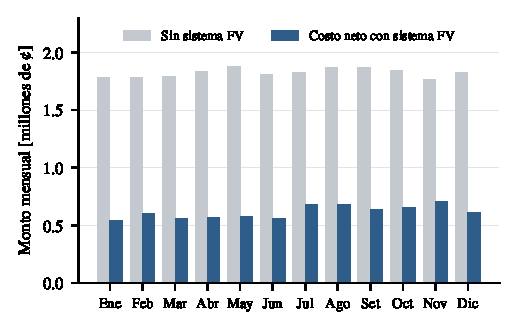
\includegraphics[width=\anchofig]{facturacion.pdf}
\caption{Factura mensual sin el sistema y con el sistema, con cargos de 2026.}
\label{fig:facturacion}
\end{figure}

\subsection{Flujo de caja e indicadores}

El flujo de caja se proyectó con los supuestos de la Tabla~\ref{tab:supuestos}, para el pago de contado y para el caso en que se financia el 80\,\% con un préstamo. La Tabla~\ref{tab:indicadores} presenta el valor presente neto (VPN), la tasa interna de retorno (TIR), el índice de rentabilidad (IR, valor presente de los flujos entre la inversión) y el período de recuperación (PRI).

La tasa de descuento de 7\,\% es un supuesto que representa el costo de oportunidad del dinero para la cooperativa: es mayor que la tasa básica pasiva, de 3.59\,\% en setiembre de 2026 \cite{bccr_tbp}, y similar a la tasa activa promedio de los créditos en colones para comercio, de 6.6\,\% \cite{bccr_tan}. Para el préstamo se supuso un interés de 9\,\%, entre las tasas activas para comercio (6.6\,\%) y para servicios (11.7\,\%) \cite{bccr_tan}, a 120 meses y con el 80\,\% financiado, condiciones similares a las ofrecidas para financiar paneles solares en el país \cite{bancopopular, avolta}.

\begin{table}[!htb]
\caption{Supuestos del flujo de caja}
\label{tab:supuestos}
\centering
\footnotesize
\setlength{\tabcolsep}{3pt}
\begin{tabular}{l l}
\toprule
Parámetro & Valor \\
\midrule
Horizonte / tasa de descuento & 25 años / 7\,\% \\
Aumento anual de tarifas y gastos & 0\,\% (base) y 3\,\% \\
Degradación (solo energía) & 1\,\% (año 1); 0.35\,\%/año \\
Mantenimiento y reposición & 1\,\% del precio por año \\
Préstamo & 80\,\% a 9\,\% anual, 120 cuotas \\
Cuota mensual del préstamo & ¢\num{1206419} \\
\bottomrule
\end{tabular}
\end{table}

\begin{table}[!htb]
\caption{Indicadores económicos (25 años)}
\label{tab:indicadores}
\centering
\footnotesize
\setlength{\tabcolsep}{3pt}
\begin{tabular}{l c S[table-format=2.1] S[table-format=2.1] S[table-format=1.2] S[table-format=2.1]}
\toprule
{Pago} & {Aumento} & {VPN} & {TIR} & {IR} & {PRI} \\
 & {anual} & {[M¢]} & {[\%]} & & {[años]} \\
\midrule
Contado (proyecto) & 0\,\% & 29.5 & 9.7 & 1.25 & 9.2 \\
Contado (proyecto) & 3\,\% & 75.6 & 12.6 & 1.63 & 8.2 \\
Préstamo (aporte propio) & 0\,\% & 23.0 & 10.7 & 1.97 & 13.1 \\
Préstamo (aporte propio) & 3\,\% & 69.1 & 16.0 & 3.90 & 11.2 \\
\bottomrule
\end{tabular}
\\[2pt]
{\footnotesize Con préstamo, la inversión inicial de los propietarios es de ¢23.81 millones. Los indicadores del proyecto y los del aporte propio tienen bases distintas y no se comparan entre sí.}
\end{table}

En el flujo de caja, la degradación del 1\,\% se aplica desde el primer año y el ahorro del año 1 queda en ¢14.38 millones; al restar el mantenimiento, el flujo neto es de ¢13.19 millones. En el caso base, pagando de contado, la inversión se recupera en 9.2 años, la TIR (9.7\,\%) supera la tasa de descuento y cada colón invertido devuelve 1.25 colones en valor presente. Con préstamo, la cuota anual (¢14.48 millones) es mayor que el flujo neto, por lo que durante los diez años del crédito el flujo es negativo, de unos ¢1.3 millones por año y la recuperación se extiende a 13.1 años (Fig.~\ref{fig:flujo}); este plazo se mide sobre el aporte propio de ¢23.81 millones y no sobre el precio total del sistema.

\begin{figure}[!htb]
\centering
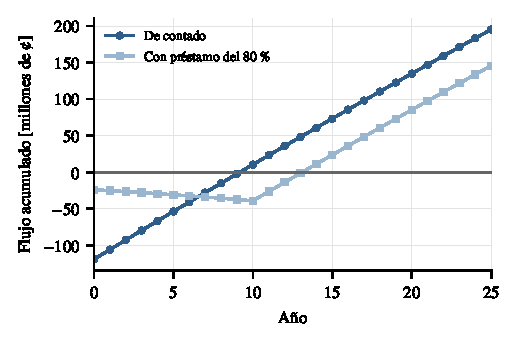
\includegraphics[width=\anchofig]{flujo_acumulado.pdf}
\caption{Flujo de caja acumulado sin aumento de tarifas.}
\label{fig:flujo}
\end{figure}

La Tabla~\ref{tab:sensibilidad} muestra cómo cambian los resultados de contado al variar los supuestos con mayor incertidumbre. Los escenarios que más cambian el resultado son los de los excedentes: como cerca de la mitad de la generación se deposita en la red, el VPN se vuelve negativo si esa energía se vende a \SI{27.40}{¢/kWh} o no se reconoce. Como escenario hipotético también se evaluó una tarifa de acceso de \SI{25}{¢/kWh} sobre la energía devuelta, que hoy no aplica a la T-CO; con ella el VPN bajaría a ¢3.7 millones. En cuanto al perfil de carga, con una carga diurna del 50\,\% de la demanda el autoconsumo baja al 41\,\% de la generación. Como la energía que deja de consumirse se deposita en la red, el ahorro disminuye solo un 9\,\%, pero el VPN se reduce a la mitad (¢14.6 millones). Por último, la tasa de descuento y el precio del sistema son supuestos sin fuente pública: con una tasa de 9\,\% o un precio 15\,\% mayor, el VPN baja a ¢6.5 y ¢9.5 millones, aunque sigue positivo.

La reducción de la demanda facturada se presenta solo como sensibilidad, porque ocurriría únicamente si la generación coincide con el intervalo en que se registra el máximo del mes, lo que no puede comprobarse sin mediciones horarias.

\begin{table}[!htb]
\caption{Sensibilidad de los resultados (contado, sin aumento de tarifas)}
\label{tab:sensibilidad}
\centering
\footnotesize
\setlength{\tabcolsep}{3pt}
\begin{tabular}{l S[table-format=2.2] S[table-format=-2.1] S[table-format=2.1] S[table-format=2.1]}
\toprule
{Escenario} & {Ahorro} & {VPN} & {TIR} & {PRI} \\
 & {[M¢]} & {[M¢]} & {[\%]} & {[años]} \\
\midrule
Caso base (medición neta) & 14.53 & 29.5 & 9.7 & 9.2 \\
Demanda facturada $-10$\,\% & 15.15 & 36.7 & 10.3 & 8.7 \\
Demanda facturada $-20$\,\% & 15.77 & 44.0 & 10.9 & 8.4 \\
Neteo con tarifa de acceso & 12.20 & 3.7 & 7.3 & 11.2 \\
Venta de excedentes & 10.24 & -18.6 & 5.2 & 13.7 \\
Excedentes sin reconocimiento & 7.89 & -44.6 & 2.3 & 18.7 \\
Carga diurna: 50\,\% de $D$ & 13.20 & 14.6 & 8.4 & 10.2 \\
Carga diurna: 65\,\% de $D$ & 14.21 & 25.9 & 9.4 & 9.4 \\
Carga diurna: 85\,\% de $D$ & 14.72 & 31.6 & 9.9 & 9.0 \\
Tasa de descuento 5\,\% & 14.53 & 59.9 & 9.7 & 9.2 \\
Tasa de descuento 9\,\% & 14.53 & 6.5 & 9.7 & 9.2 \\
Precio del sistema $+15$\,\% & 14.53 & 9.5 & 7.8 & 10.7 \\
\bottomrule
\end{tabular}
\\[2pt]
{\footnotesize $D$: demanda facturada del mes. Caso base: 75\,\% de $D$.}
\end{table}

\subsection{Comparación con otras potencias}\label{sec:alternativas}

Para conocer cómo cambia la rentabilidad con el tamaño, la Tabla~\ref{tab:alternativas} compara el sistema seleccionado con sistemas de menor potencia, formados con cadenas completas de 17 módulos y evaluados con el mismo modelo.

\begin{table*}[!htb]
\caption{Comparación de potencias (año 1, medición neta sencilla)}
\label{tab:alternativas}
\centering
\footnotesize
\setlength{\tabcolsep}{5pt}
\begin{tabular}{S[table-format=3.1] c c S[table-format=1.2] S[table-format=3.1] S[table-format=2.1] S[table-format=2.1] S[table-format=2.2] S[table-format=2.1] S[table-format=2.1] S[table-format=2.1]}
\toprule
{$P_{fv}$} & {Cadenas} & {Inversores} & {DC/AC} & {Inversión} & {Gen./Cons.} & {Depositada} & {Ahorro} & {VPN} & {TIR} & {PRI} \\
{[kWp]} & & {(kW AC)} & & {[M¢]} & {[\%]} & {[\% Gen.]} & {[M¢]} & {[M¢]} & {[\%]} & {[años]} \\
\midrule
76.5 & $10\times17$ & 2 (50 kW) & 1.53 & 52.5 & 44.7 & 12.6 & 6.72 & 16.5 & 10.4 & 8.7 \\
107.1 & $14\times17$ & 3 (75 kW) & 1.43 & 74.7 & 62.6 & 27.9 & 9.42 & 21.9 & 10.2 & 8.8 \\
137.7 & $18\times17$ & 4 (100 kW) & 1.38 & 95.9 & 80.5 & 39.9 & 12.12 & 28.3 & 10.2 & 8.8 \\
153.0 & $20\times17$ & 4 (100 kW) & 1.53 & 103.2 & 89.3 & 44.6 & 13.38 & 34.4 & 10.6 & 8.6 \\
168.3 & $22\times17$ & 5 (125 kW) & 1.35 & 119.0 & 98.4 & 48.8 & 14.53 & 29.5 & 9.7 & 9.2 \\
\bottomrule
\end{tabular}
\\[2pt]
{\footnotesize Gen./Cons.: generación anual respecto al consumo (\SI{223.0}{MWh}). Depositada: energía entregada a la red respecto a la generación. Ahorro del año 1 sin degradación. VPN a 25 años con tasa de 7\,\%, pago de contado y sin aumento de tarifas. Para 107.1, 137.7 y \SI{153}{kWp}, el alimentador y sus protecciones se estimaron por escalamiento.}
\end{table*}

Con la medición neta, el ahorro crece casi en proporción a la potencia, porque la energía depositada se recupera más adelante. Todas las alternativas tienen un VPN positivo y una TIR cercana al 10\,\%. El sistema de \SI{153}{kWp} tiene el VPN más alto, porque el de \SI{168.3}{kWp} necesita un quinto inversor y protecciones de mayor capacidad para un 10\,\% más de generación; la diferencia es de ¢4.9 millones de VPN y 0.9 puntos de TIR, y se mantuvo la propuesta de \SI{168.3}{kWp} porque su generación anual se acerca más al consumo del establecimiento.
